\section{Graph Summary for Web Data Management}
\label{chap03:sec:wd-mgnt}

The graph summary highlights the structure of a graph, which in the case of RDF data consists in the use of predicates, classes, and their relationships. As such, a graph summary exhibits a similar function as that of a \emph{schema}. In comparison to the VoID~\cite{alexander:2009:dld} approach, the use of a graph summary as a schema provides additional information, e.g., which predicates co-occur, or how are the classes in a dataset inter-connected.

We define a graph schema model on top of a graph summary in Section~\ref{chap03:sec:gschema}. We describe a RDF model for a graph summary in Section~\ref{chap03:summary-rdf}.

\subsection{Graph Schema}
\label{chap03:sec:gschema}

In order to use the information in a graph effectively, it is necessary to have at disposition a schema of that graph. The schema provides a description of the structure of the entity graph. Given a graph schema, it is then possible to understand how the data is modelled so that it is possible to perform meaningful operations such as querying, optimising query execution, or partitioning data.% \todo{add refs}

The schema of the entity graph is itself a graph as in \cite{kunii1983graph}, where a model for defining integrity constraints and similar rules as in a traditional relational database schema is proposed. In this work, we focus on the structural description of the graph.% We consider the schema as a graph where there is a \emph{simulation} from the entity graph to that schema \cite{wang:2000:ags}. We refer to the schema of the entity graph simply as the \emph{graph schema}. \todo{Review mention of simulation}

\subsection{Overview}

Knowledge is commonly represented using directed graphs, as it is expressive enough for modelling data with complex relationships. For example, semantic networks~\cite{sowa2006semantic} have been used in artificial intelligence and machine translation, with the Web of Data being a large scale instance.

Similarly to schemas in databases, there exists \emph{graph schemas} which defines the structure of the graph. A graph schema can be pre-defined as in a top-down approach, or can be generated from the data itself in a bottom-up approach. Thanks to a graph schema, the potential benefits are numerous: optimisation of query processing, data integration, data discovery, etc.

There exists two approaches for creating a graph schema, each sitting at opposite extremities as depicted by Figure~\ref{fig:introduction:schema-tradeoffs}. On the right side, we have the top-down approaches where a person creates the schema manually. Such a hand-crafted schema ensures the data to be conform with it, but at the cost of less flexibility with regards to the evolution of the schema in time and its customisation to specific needs.

On the left side, we have the bottom-up approaches which rely only on the data. Such schemas offer more flexibility when manipulating the data, but they offer more heterogeneous information.
Indeed, a hand-crafted is the result of a careful thought-process, while a generated (bottom-up approach) schema is susceptible to data heterogeneity.

\begin{figure}
	\centering
	\resizebox{.6\textwidth}{!}{
		\begin{tikzpicture}
\node (bt) at (0,.5) {Bottom-Up};
\node (td) at (5,.5) {Top-Down};
\draw [|-|,thick] (0,0) -- (5,0);

\node at (-1,-.75) {\emph{Flexibility}};
\draw [fill=black,path fading=east] (0,-.5) -- (5,-.75) -- (0,-1) -- cycle;

\node at (6,-1.5) {\emph{Accuracy}};
\draw [fill=black,path fading=west] (0,-1.5) -- (5,-1.25) -- (5,-1.75) -- cycle;
\end{tikzpicture}

	}
	\caption{Trade-offs between graph schema creation approaches.}
	\label{fig:introduction:schema-tradeoffs}
\end{figure}

\subsubsection{Top-Down Graph Schema}

The structure of the graph can be rigorously defined. In \cite{kunii1983graph} the schema of the database is itself represented as a graph, which facilitates the construction of the database as well as the query formulation. In \cite{antoniou2004web} the authors present the Web Ontology Language which represents the ontology layer in the Semantic Web stack. It allows to define classes, properties, and relationships between classes. Regarding XML data, a graph schema can be expressed via \emph{XML Schemas}\footnote{XMLSchema: \url{http://www.w3.org/XML/Schema}}. In these methods, the graph data either has to be squeezed to fit the pre-defined schema, or the schema has to be updated to meet the new requirements. Updating the schema is an expensive operation, since the graph schemas are generally complex.

\subsubsection{Bottom-Up Graph Schema}

In a bottom-up approach, the schema is generated from the data itself by using some features of the data, e.g., attributes of a node. In order to generate a schema, the process must then preserve the \emph{structure} of the graph. %Such a process is called a \emph{graph homomorphism}, i.e., a mapping from the data to the graph schema where every adjacent nodes in the data are mapped to adjacent nodes in the graph schema. The Figure~\ref{fig:introduction:homomorph} depicts a graph that is homomorphic to the graph in Figure~\ref{fig:introduction:graph}, which is then called the \emph{schema} of that graph.
This can be achieved by using a summarisation relation. As such, we can use a graph summary to fulfil the function of a schema.

%The authors in \cite{goldman1997dataguides} propose \emph{DataGuides}, a method based on automata equivalence which allows to generate a concise and accurate graph schema. However, due to the structural heterogeneity of the graph, the generated graph schema may be large or even larger than the data itself, as discussed in \cite{goldman1999approximate}. In order to counter-balance this, some techniques allow some errors in the graph so to keep the graph schema concise, e.g., \cite{chen:2003:dia,navlakha:2008:gsb}. For example, although the graph in Figure~\ref{fig:introduction:homomorph} shows a path from the node 3 to the node 2 via 1, there is no such path in the graph of Figure~\ref{fig:introduction:graph}.

%\begin{figure}
%	\centering
%	\begin{subfigure}[b]{.4\textwidth}
%		\centering
%		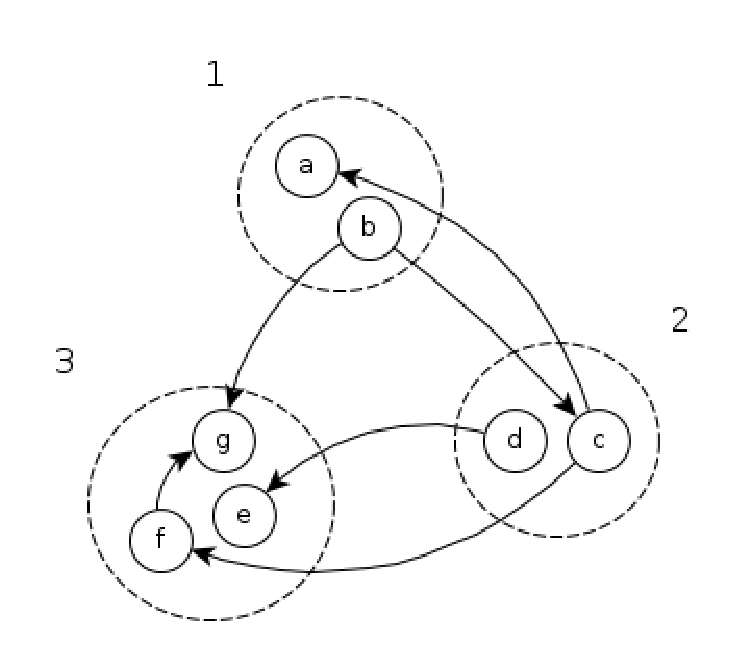
\includegraphics[scale=0.5]{01-introduction/figures/homomorphism1}
%		\caption{A data graph. Nodes within a dashed circle are mapped to a same node.}
%		\label{fig:introduction:graph}
%	\end{subfigure}
%	\quad
%	\begin{subfigure}[b]{.45\textwidth}
%		\centering
%		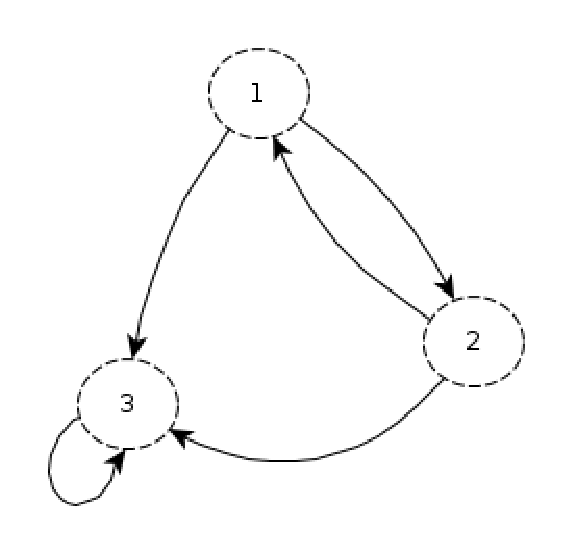
\includegraphics[scale=.5]{01-introduction/figures/homomorphism2}
%		\caption{A graph homomorphic to the graph in Figure~\ref{fig:introduction:graph}}
%		\label{fig:introduction:homomorph}
%	\end{subfigure}
%	\caption{Graph schema based on a graph homomorphism.}
%\end{figure}

\subsubsection{Graph Schema Granularity}

There is a need for schemas of varying granularity. It is common for database schemas to be large and therefore difficult for users to understand. The authors in \cite{yu:2006:schema-summarization,yang:2011:summary-graphs} proposed methods for summarizing the information in schemas in order to highlight the ``important'' parts. This shows that applications having different degree of interactivity with the data require different parts to be focused, while others can be hidden. We call this notion as the \emph{granularity level} of the schema.

%By altering the mappings in the graph homomorphism, the resulting schema is then more or less coarse, i.e., it carries more or less information about the data. For instance in Figure~\ref{fig:introduction:graph}, if the two nodes $a$ and $b$ were mapped to different nodes in the schema, the latter would be finer grained than the schema in Figure~\ref{fig:introduction:homomorph}, since the path from node 2 to 3 via node 1 would not exist.
A varying level of granularity can be achieved by modifying appropriately the summarisation relation of a graph summary. By altering the mappings of the relation, the resulting schema is then more or less coarse, i.e., it carries more or less information about the data. The granularity can be varied through the use of the presented summarisation relations in Section~\ref{sec:approximate}. How coarse a granularity is can be measured thanks to the graph summary precision model introduced in Chapter~\ref{chap03:sec:quality}.

%\subsection{Abstract Model}
%\label{sec:gschema:abstract-model}
%
%The graph schema is a graph that describes the structure of the entity graph $G$. It informs on the types used, the relations between types, and the attributes associated with a type.
%%The graph schema is a layer located between the entity and the dataset layers. There can be more than one graph schema for a given entity graph, with each providing more or less details about the structure of the entity graph.
%Although the schema is represented as a graph, its elements carry a different semantics than in an entity graph. The reason is that the schema describes the structure of the entity graph. A node in a graph schema represents a \emph{collection} of nodes in the entity graph. Furthermore, it can be associated with attributes and types information, derived from the entities it is composed of. An edge in a graph schema represents a \emph{set} of edges in the entity graph that connect entities together.
%
%\begin{quote}
%	The Figure~\ref{fig:schema-graphs} depicts two possible graph schemas for Figure~\ref{fig:graph}. A node in a graph schema reports on the left column the type, on the right the attribute, and on the bottom row are indicated the entities of the figure it contains.
%	The schema on Figure~\ref{fig:sg1} is minimal, it consists of a single node with all the edges appearing in the entity graph adjacent to it. Although it is a valid graph schema, it does not however give any insight in the entity graph beyond what attributes and what types are used.
%	A deeper insight is achieved with the schema on Figure~\ref{fig:sg2} generated by grouping entities based on their type feature, e.g., we observe that a Person is connected to a City via the link ``lives''.
%\end{quote}
%
%While generating a graph schema, it is possible to gather statistics about the data. For example, we can count the number of entities a node of the schema contains, or how many times a certain attribute is used. The accumulation of such statistics can be used for various purpose, e.g., browsing the most used parts of the data.
%
%\begin{figure}
%	\centering
%	\begin{subfigure}{.42\textwidth}
%		\centering
%		\resizebox{\textwidth}{!}{
%			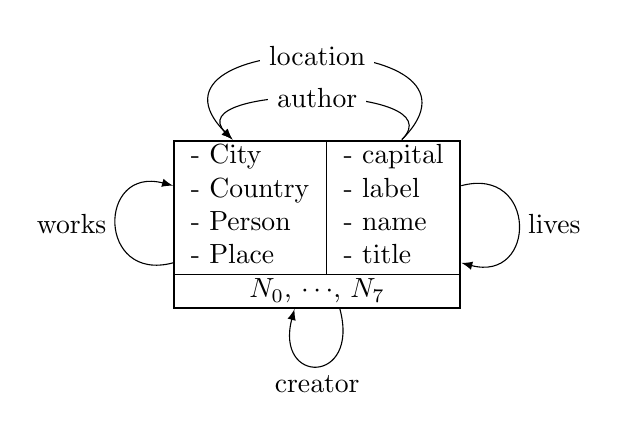
\begin{tikzpicture}[>=latex]
\node (T) [draw,thick,rectangle, inner sep=0pt] {
\begin{tabular}{l|l}
- City & - capital \\
- Country & - label \\
- Person & - name \\
- Place & - title \\
\hline
\multicolumn{2}{c}{$N_0$, $\cdots$, $N_7$}
\end{tabular}
};
\draw [loop, distance=2cm,->] (T) to node [fill=white] {location} (T);
\draw [loop, distance=1cm,->] (T) to node [fill=white] {author} (T);
\draw [loop below, distance=1cm,->] (T) to node {creator} (T);
\draw [loop right, distance=1cm,->] (T) to node {lives} (T);
\draw [loop left, distance=1cm,->] (T) to node {works} (T);
\end{tikzpicture}
%		}
%		\caption{A simple graph schema}
%		\label{fig:sg1}
%	\end{subfigure}
%	\quad
%	\begin{subfigure}{.54\textwidth}
%		\centering
%		\resizebox{\textwidth}{!}{
%			\begin{tikzpicture}[>=latex]
\node (city) [draw,thick,rectangle,inner sep=0] {
\begin{tabular}{l|l}
- City & - label \\
\hline
\multicolumn{2}{c}{$N_3$}
\end{tabular}
};
\node (country) [draw,thick,rectangle,inner sep=0, right = 2.5cm of city] {
\begin{tabular}{l|l}
- Country & - capital \\
 & - label \\
\hline
\multicolumn{2}{c}{$N_6$, $N_7$}
\end{tabular}
};
\node (person) [draw,thick,rectangle,inner sep=0,above = 1.5cm of city] {
\begin{tabular}{l|l}
- Person & - name \\
\hline
\multicolumn{2}{c}{$N_1$, $N_2$}
\end{tabular}
};
\node (place) [draw,thick,rectangle,inner sep=0,above =1.5cm of country] {
\begin{tabular}{l|l}
- Place & - capital \\
 & - label \\
\hline
\multicolumn{2}{c}{$N_4$, $N_5$, $N_6$, $N_7$}
\end{tabular}
};
\node (pub) [draw,thick,rectangle,inner sep=0,above = of person] {
\begin{tabular}{l|l}
$\varnothing$ & - title \\
\hline
\multicolumn{2}{c}{$N_0$}
\end{tabular}
};

\draw [->] (person) to node [fill=white] {lives} (city);
\draw [->] (person) to node [fill=white] {works} (place);
\draw [->] (city) to node [fill=white] {location} (place);
\draw [->] (city) to node [fill=white] {location} (country);
\draw [->] (place) to node [fill=white] {location} (country);
\draw [loop,distance=2cm,->] (place) to node [fill=white] {location} (place);
\draw [bend left=50,->] (pub) to node [fill=white] {author} (person);
\draw [bend right=50,->] (pub) to node [fill=white] {creator} (person);

\end{tikzpicture}
%		}
%		\caption{A graph schema based on the \emph{Types} summarisation relation $R_t$}
%		\label{fig:sg2}
%	\end{subfigure}
%	\caption{Two possible graph schemas for Figure~\ref{fig:graph}. The left columns report the type information of a node, while the right the attribute. The bottom row of a node indicates the entities of the figure it contains.}
%	\label{fig:schema-graphs}
%\end{figure}
%
%\subsection{Formal Model}
%\label{sec:gschema:formal-model}
%
%A graph schema is a graph where there is a \emph{simulation} from the entity graph to that graph schema \cite{wang:2000:ags}. In other words, every path and combination of paths that appear in the entity graph must also appear in the graph schema.
%
%\begin{quote}
%	For example, the entity graph in Figure~\ref{fig:graph} depicts the node $N_1$ of type Person that has three attributes, i.e., lives, name, and works. Both graph schemas in Figure~\ref{fig:schema-graphs} show such a pattern.
%\end{quote}
%
%Each node of the entity graph is mapped to a node in the graph schema; we say then that the entity graph is \emph{simulated by} the graph schema.
%
%\begin{definition}[Simulation]
%	Let $G_1 = \left\langle V_1, A_1, l_{v_1} \right\rangle$ and $G_2 = \left\langle V_2, A_2, l_{v_2} \right\rangle$ be two graphs. A relation $R$ from $V_1$ to $V_2$ is a simulation if it satisfies
%	\begin{equation*}
%	\begin{split}
%	& \forall \alpha \in A_1,\: \forall (x_1,y_1) \in V^2_1,\: \forall x_2 \in V_2 \\
%	&\begin{aligned}
%	\left(x_1 \overset{\alpha}{\rightarrow} y_1 \wedge x_1 R x_2 \implies \exists y_2 \in V_2 \left( y_1 R y_2 \wedge x_2 \overset{\alpha}{\rightarrow} y_2 \right) \right)
%	\end{aligned}
%	\end{split}
%	\end{equation*}
%	\label{eq:simulation}
%\end{definition}
%
%For a relation $R$ to be a \emph{simulation} from the nodes of the graph $G_1$ to $G_2$, it is required that for all edges in $G_1$, there exists a corresponding edge in $G_2$. The Figure~\ref{fig:simulation} depicts the Definition~(\ref{eq:simulation}). The dotted arrows represent the missing requirements for $R$ to be a simulation:
%\begin{enumerate}
%	\item there exists an edge labelled $\alpha$ that links $x_2$ to $y_2$; and
%	\item there is a $R$ relation between the nodes $y_2$ and $y_1$.
%\end{enumerate}
%The definition presents a recursive aspect. The recursion is stopped if a leaf node is met, since two leaf nodes are in simulation. For example in Figure~\ref{fig:simulation}, if the nodes $y_1$ and $y_2$ were literals in the RDF modelling, then there would be a simulation relation between $x_1$ and $x_2$ since both have an attribute $\alpha$ that lead to a leaf node.
%
%A graph schema is \emph{valid} with regards to the entity graph if there exists a simulation from the nodes of the entity graph to those of the graph schema.
%
%\begin{figure}
%	\centering
%	\begin{tikzpicture}[->,>=stealth']
% G1
\draw (2,3) ellipse (50pt and 22pt);
\draw (0,3.5) node {$G_1$};

\draw (1,3) circle (10pt);
\node (x1) at (1,3) {$x_1$};

\draw (3,3) circle (10pt);
\node (y1) at (3,3) {$y_1$};

\draw [->] (1.35,3) -- node[auto]{$\alpha$} (2.65,3);

% G2
\draw (2,1) ellipse (50pt and 22pt);
\draw (0,1.5) node {$G_2$};

\draw (1,1) circle (10pt);
\node (x2) at (1,1) {$x_2$};

\draw (3,1) circle (10pt) [dashed];
\node (y2) at (3,1) {$y_2$};

\draw [dashed,->] (1.35,1) -- node[auto]{$\alpha$} (2.65,1);

% simulation
\draw [->] (1,2.65) to [bend right=45] node[swap,auto]{$R$} (1,1.35);

\draw [->,dashed] (3,2.65) to [bend left=45] node[auto]{$R$} (3,1.35);

\end{tikzpicture}
%	\caption{Depiction of the simulation Definition~(\ref{eq:simulation}).}
%	\label{fig:simulation}
%\end{figure}

%\subsection{Schema Accuracy}
%
%A graph schema describes the structure of the entity graph. From the simulation relation, we know that any path occurring in the data appears in the schema as well. However, the opposite may not always be true. It is possible to draw some conclusions about the data by observing the schema that may actually be wrong. By wrong, we mean that a graph pattern occurs in the schema, but not in the data. This generally stems from the data heterogeneity, i.e., a loose use of a variety of vocabularies.
%
%The schema graph in Figure~\ref{fig:sg2} depicts two nodes, one with type \emph{Place} and the other with \emph{Country}. For both, it reports \emph{capital} and \emph{label} as attributes. However, there is no entity in the data depicted in Figure~\ref{fig:graph} of either type that have both attributes. The reason is that both nodes represent the aggregation of several entities, i.e., $N_4$, $N_5$, $N_6$, and $N_7$ for the one typed \emph{Place}, and $N_6$, $N_7$ for the other.

\subsection{Representation of Graph Summaries}
\label{chap03:summary-rdf}

In this section, we present a RDF model for describing a graph summary. This allows the summary to be queried as any other RDF graph, ultimately so it can be used in conjunction with the entity graph.

Viewing the graph summary as a RDF graph requires the creation of URIs for identifying sumnodes and sumedges. A URI for a sumnode can be created based on the features the summarisation relation it is based on, e.g., on the type information for the \emph{Types} summary $R_t$. The sumedge URI can be created by considering the source and target sumnodes, as well as the attribute.

\begin{remark}
	Although an edge is represented with a single statement in RDF, this is not the case for a sumedge of the summary if we need to associate with it metadata, e.g., statistics or the sumedge provenance. Therefore, we need to describe formally the sumedge.

	For example, consider the sumedge ``\emph{:Person :writes :Book .}'', represented as a triple, which relates the sumnode ``:Person'' to the sumnode ``:Book''. If we need to associate a statistic to that sumedge, we need to RDFify it with four triples:
	\begin{enumerate}
		\item \emph{:se :source :Person .}
		\item \emph{:se :target :Book .}
		\item \emph{:se :label :writes .}
		\item \emph{:se :statistic "1" .}
	\end{enumerate}
	where ``:se'' is the URI for that sumedge, the first triple describes the source, the second the target, the third the label of the sumedge, and the fourth the statistic associated to that triple.
\end{remark}

We depict in Figures~\ref{fig:rdf-node}~and~\ref{fig:rdf-edge} the ontology of the summary RDF model of the sumnode and sumedge respectively, where the label of a node indicates the type of that node. For example, the range of the origin predicate is \emph{xsd:anyURI}. In Figure~\ref{fig:rdf-node} the dot represents an intermediate node, which can be translated into a blank node in the RDF model. We describe in the Table~\ref{tab:rdf-terms} the vocabulary terms.\\

In the case where a summary describes a collection of inter-linked datasets, we record the provenance of the summarised edges at the sumnode (resp., sumedge) level using the predicate \emph{origin}. The predicate \emph{label} indicates the type or attribute associated to a sumnode (resp., sumedge). We record the features of the summarisation relation, e.g., a type for the \emph{Types} summary $R_t$, using the predicate \emph{feature}. In case of a summarisation relation that is based on the type feature, we record as well the attribute type that defined that type.

\subsubsection{Reification of the sink sumnode $\varnothing$.}

There exists several ways to reify the sink sumnode $\varnothing$ which represents abstracted data from the entity graph, e.g., literals and URIs with no outgoing edge. We represent it in the RDF summary as an empty literal. Another solution would be to not represent it at all.

\begin{figure}
	\centering
	\begin{subfigure}[b]{.45\textwidth}
		\centering
		\resizebox{\textwidth}{!}{
			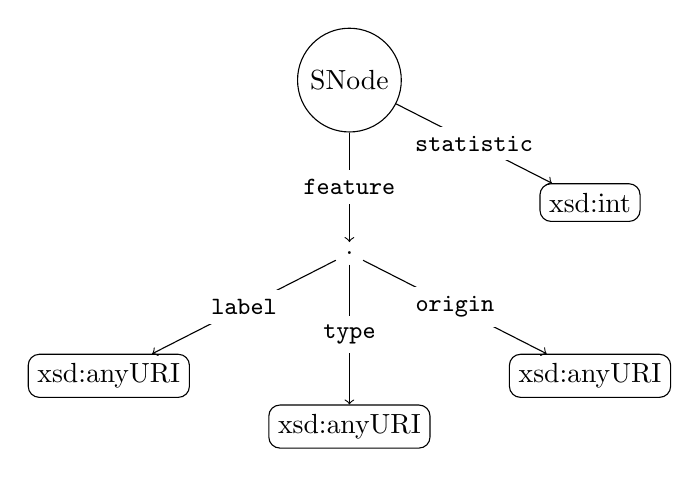
\begin{tikzpicture}[->,node/.style={draw,circle},leaf/.style={draw,rounded corners},node distance=2.2cm]

\node[node] (node) {SNode};
\node[leaf,below right of = node,xshift=1.5cm] (card) {xsd:int};
\node[below of = node] (type) {.};
\node[leaf,below left of = type,xshift=-1.5cm] (typelabel) {xsd:anyURI};
\node[leaf,below right of = type,xshift=1.5cm] (torigin) {xsd:anyURI};
\node[leaf,below of = type] (ttype) {xsd:anyURI};

\path[every node/.style={font=\small\ttfamily,fill=white}]
(node)	edge node {statistic} (card)
			edge node {feature} (type)
(type)	edge node {label} (typelabel)
			edge node {origin} (torigin)
			edge node {type} (ttype)
;
\end{tikzpicture}
		}
		\caption{Node class}
		\label{fig:rdf-node}
	\end{subfigure}
	\quad
	\begin{subfigure}[b]{.35\textwidth}
		\centering
		\resizebox{\textwidth}{!}{
			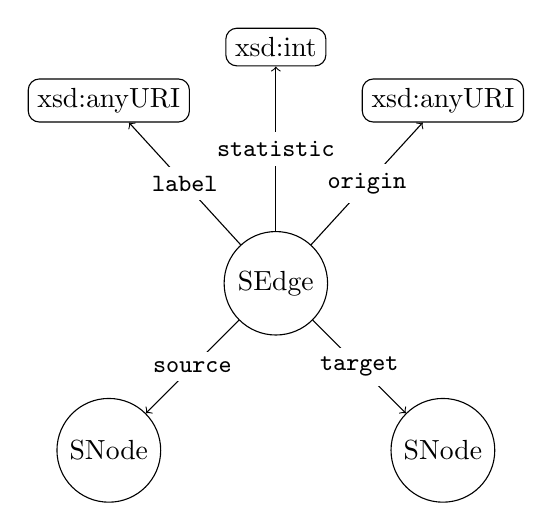
\begin{tikzpicture}[->,node/.style={draw,circle},leaf/.style={draw,rounded corners},node distance=3cm]

\node[node] (edge) {SEdge};
\node[node,below left of = edge] (source) {SNode};
\node[node,below right of = edge] (target) {SNode};
\node[leaf,above left of = edge,yshift=.2cm] (label) {xsd:anyURI};
\node[leaf,above of = edge] (card) {xsd:int};
\node[leaf,above right of = edge,yshift=.2cm] (origin) {xsd:anyURI};

\path[every node/.style={fill=white,font=\small\ttfamily}]
(edge)	edge node {source} (source)
			edge node {target} (target)
			edge node {label} (label)
			edge node {statistic} (card)
			edge node {origin} (origin)
;
\end{tikzpicture}
		}
		\caption{Edge class}
		\label{fig:rdf-edge}
	\end{subfigure}
	\qquad
	\begin{subfigure}[b]{\textwidth}
		\resizebox{\textwidth}{!}{
			\begin{tabular}{lc@{\hs}l}
				\toprule
				& \phantom{a} & \multicolumn{1}{c}{Description} \\
				\cmidrule{3-3}
				\underline{\textbf{Class}} & & \\
				SEdge & \phantom{a} & This class refers to a sumedge $(x, \alpha, y) \in \mathcal{B}$ of the summary. \\
				SNode & \phantom{a} & This class refers to a sumnode $x \in \mathcal{W}$ of the summary. \\
				\midrule
				\underline{\textbf{Predicate}} & & \\
				feature & \phantom{a} & A feature of the summarisation relation. \\
				label & \phantom{a} & The label associated with a sumnode or a sumedge, i.e., either an attribute or a type. \\
				origin & \phantom{a} & The provenance of the summarised edge, or of a feature of the summarisation relation. \\
				source & \phantom{a} & The sumnode $x$ in the sumedge $(x, \alpha, y) \in \mathcal{B}$. \\
				statistic & \phantom{a} & A statistic associated with a sumnode or a sumedge, e.g., \emph{count}. \\
				target & \phantom{a} & The sumnode $y$ in the sumedge $(x, \alpha, y) \in \mathcal{B}$. \\
				type & \phantom{a} & The attribute type \gls{atype}. \\
				\bottomrule
			\end{tabular}
		}
		\caption{Vocabulary terms}
		\label{tab:rdf-terms}
	\end{subfigure}
	\caption{RDF reification of the graph summary}
	\label{fig:rdf-summary}
\end{figure}

\subsubsection{Levels of Reification}

Depending on the use of the graph summary, a subset of the presented vocabulary is needed. For example, if no statistic was computed then the predicate \emph{statistic} is not needed. In this section, we present two possible reification. A \emph{lite} reification which reifies only the structural information in the summary, and a \emph{full} reification which captures all the information made available by the graph summary.

\minisec{Full Reification}

In this level of reification, we use every vocabulary terms presented in the previous section. We note nonetheless that the \emph{origin} predicate is optional, since it is not needed in the case of summarising a single dataset.\\

Due to the RDF reification of the summary, there exists a case which might cause the summary to be larger than the original. Indeed, if the summarisation relation is a \emph{one-to-one} mapping from the entity graph to the summary, the number of RDF statements used to describe the summary might be greater than for the original graph. A single statement in the entity graph requires six statements for describing the corresponding sumedge, i.e., the five truples depicted in the Figure~\ref{fig:rdf-edge} plus one for the type attribute.

In addition to those six statements, we must also account for the statements describing the adjacent sumnodes. Depending on the application of the graph summary, the full description of the graph summary can be excessive.\\

Table~\ref{tab:reification-edge-case-full} reports the \emph{Types} summarisation of a simple entity graph for which the summarisation has a one-to-one mapping. We observe that the full reification of the summary consists of 18 triples, against 3 for the entity graph.

\minisec{Lite Reification}

For this reification, we don't retain information such as provenance or statistics. Instead, we are only concerned with the structural description of the graph. A direct consequence is that the size of the RDF summary is reduced significantly. In order to do so, we only need to create a URI for the sumnodes through object invention.

Although this reification is not as insightful as the previous one, it provides nonetheless a succinct description of the graph's structure. Table~\ref{tab:reification-edge-case-lite} reports the lite reification of the graph in Table~\ref{tab:reification-edge-case-full}.

\begin{table}
	\centering
	\begin{subfigure}{.475\textwidth}
		\centering
		\resizebox{\textwidth}{!}{
			\begin{tabular}{lllc@{\s}lll}
				\toprule
				\multicolumn{3}{c}{$G$} & \phantom{a} & \multicolumn{3}{c}{$\mathcal{S}_t$} \\
				\cmidrule{1-3} \cmidrule{5-7}
				\multirow{6}{*}{p1} & \multirow{6}{*}{\gls{atype}} & \multirow{6}{*}{Person} & \multirow{6}{*}{\phantom{a}} & t1 & $a$ & SNode \\
				& & & & t1 & statistic & 1 \\
				& & & & t1 & feature & fp1 \\
				& & & & fp1 & label & Person \\
				& & & & fp1 & type & \gls{atype} \\
				& & & & fp1 & origin & acme.org \\
				\cmidrule{1-3} \cmidrule{5-7}
				\multirow{6}{*}{p1} & \multirow{6}{*}{author} & \multirow{6}{*}{d1} & \multirow{6}{*}{\phantom{a}} & e1 & $a$ & SEdge \\
				& & & & e1 & label & author \\
				& & & & e1 & statistic & 1 \\
				& & & & e1 & origin & acme.org \\
				& & & & e1 & source & t1 \\
				& & & & e1 & target & t2 \\
				\cmidrule{1-3} \cmidrule{5-7}
				\multirow{6}{*}{d1} & \multirow{6}{*}{\gls{atype}} & \multirow{6}{*}{Document} &\multirow{6}{*}{\phantom{a}} & t2 & $a$ & SNode \\
				& & & & t2 & statistic & 1 \\
				& & & & t2 & feature & fp2 \\
				& & & & fp2 & label & Document \\
				& & & & fp2 & type & \gls{atype} \\
				& & & & fp2 & origin & acme.org \\
				\bottomrule
			\end{tabular}
		}
		\caption{Full reification. The edge $(p1, author, d1)$ is mapped to the sumedge that is reified with \emph{e1}.}
		\label{tab:reification-edge-case-full}
	\end{subfigure}
	\quad
	\begin{subfigure}{.475\textwidth}
		\centering
		\resizebox{\textwidth}{!}{
			\begin{tabular}{lllc@{\s}lll}
				\toprule
				\multicolumn{3}{c}{$G$} & \phantom{a} & \multicolumn{3}{c}{$\mathcal{S}_t$} \\
				\cmidrule{1-3} \cmidrule{5-7}
				p1 & \gls{atype} & Person & \phantom{a} & t1 & \gls{atype} & Person \\
				p1 & author & d1 & \phantom{a} & t1 & author & t2 \\
				d1 & \gls{atype} & Document & \phantom{a} & t2 & \gls{atype} & Document \\
				\bottomrule
			\end{tabular}
		}
		\caption{Lite reification.}
		\label{tab:reification-edge-case-lite}
	\end{subfigure}
	\caption{Full and lite reification of a \emph{Types} summary $R_t$. The summarisation relation $R_t$ has with the example data a one-to-one mapping from the graph $G$ to the summary $\mathcal{S}_t$. The node \emph{p1} is mapped to the sumnode \emph{t1} and \emph{d1} to \emph{t2}.}
	\label{tab:reification-edge-case}
\end{table}

%\subsection{Deploying Graph Summaries}
%\label{chap03:summary-deploy}

%In order to deploy a graph summary, we embed it into a named graph which is preferably located in the same endpoint as the original graph. In this way, the summary can be used in conjunction with the original data.
